\chapter{Appendix B: Additional Figures}

% \begin{figure}
%     \centering
%     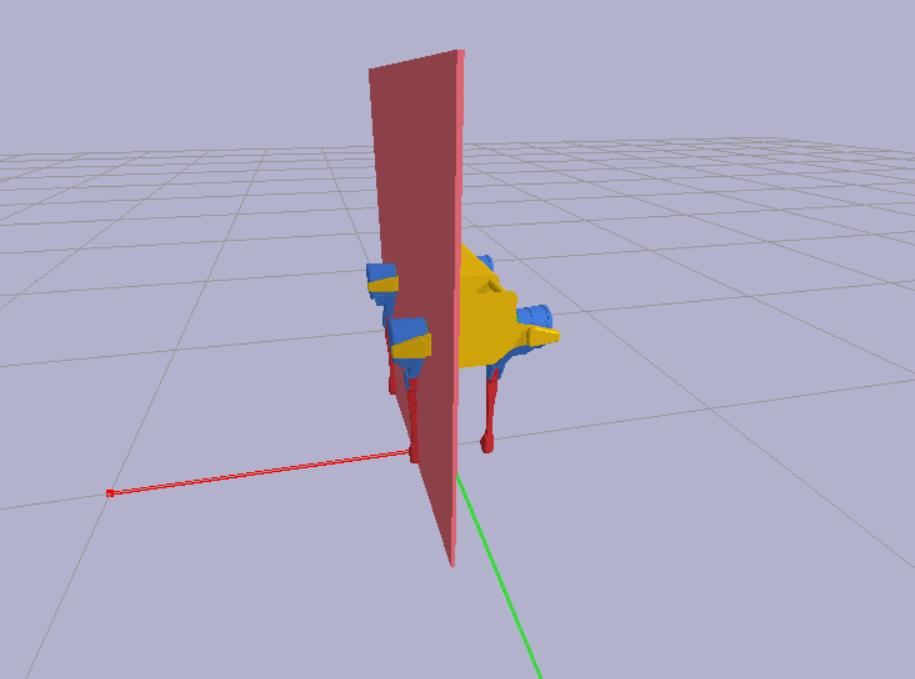
\includegraphics[width=1\textwidth]{figures/parasaggital.png}
%     \caption{Diagram of robot planes, the red square indicates the robots Parasaggital plane.}
%     \label{fig:parasaggital}
% \end{figure}
% \begin{figure}
%     \centering
%     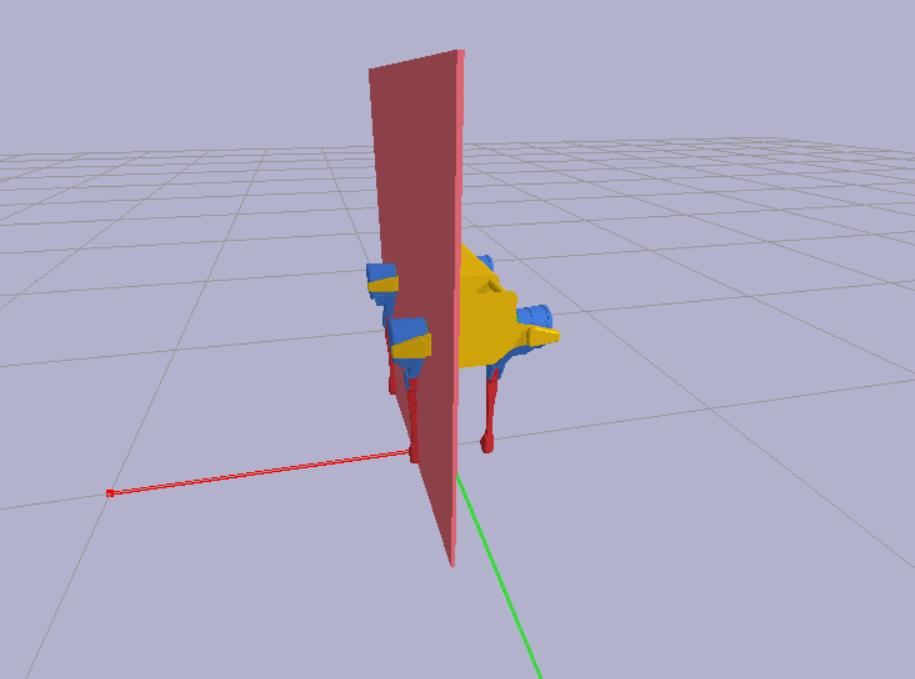
\includegraphics[width=1\textwidth]{figures/parasaggital.png}
%     \caption{Diagram of robot planes, the red square indicates the robots Parasaggital plane.}
%     \label{fig:parasaggital}
% \end{figure}
% \begin{figure}
%     \centering
%     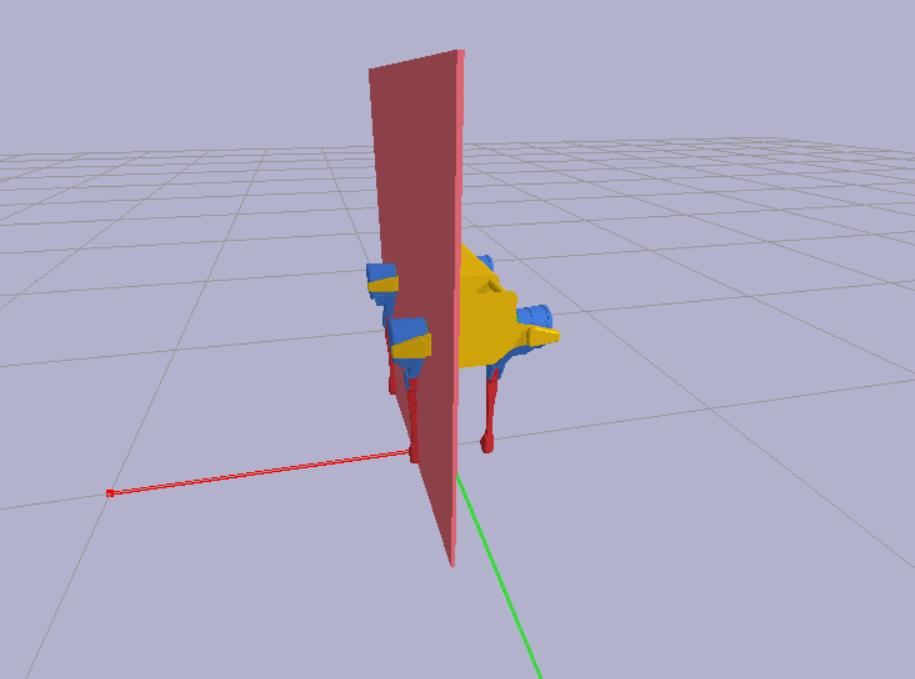
\includegraphics[width=1\textwidth]{figures/parasaggital.png}
%     \caption{Diagram of robot planes, the red square indicates the robots Parasaggital plane.}
%     \label{fig:parasaggital}
% \end{figure}

\begin{figure}[h!]
    \centering
    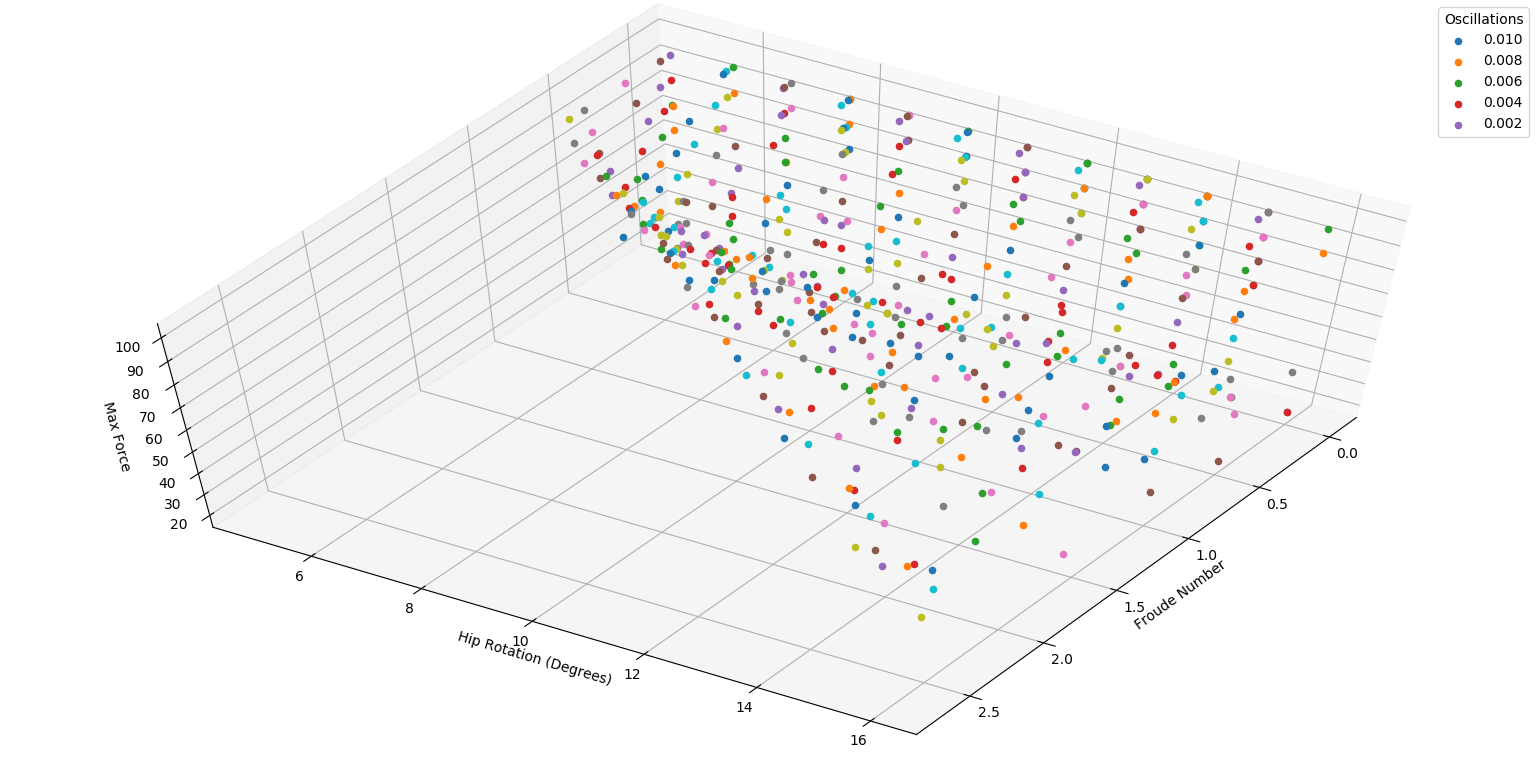
\includegraphics[width=1\textwidth]{figures/forcerotationfroude1.png}
    \label{froudenumbervsangle}
    \caption{All variation of experiments shown on 3D graph, view 1}
\end{figure}

\begin{figure}[h!]
    \centering
    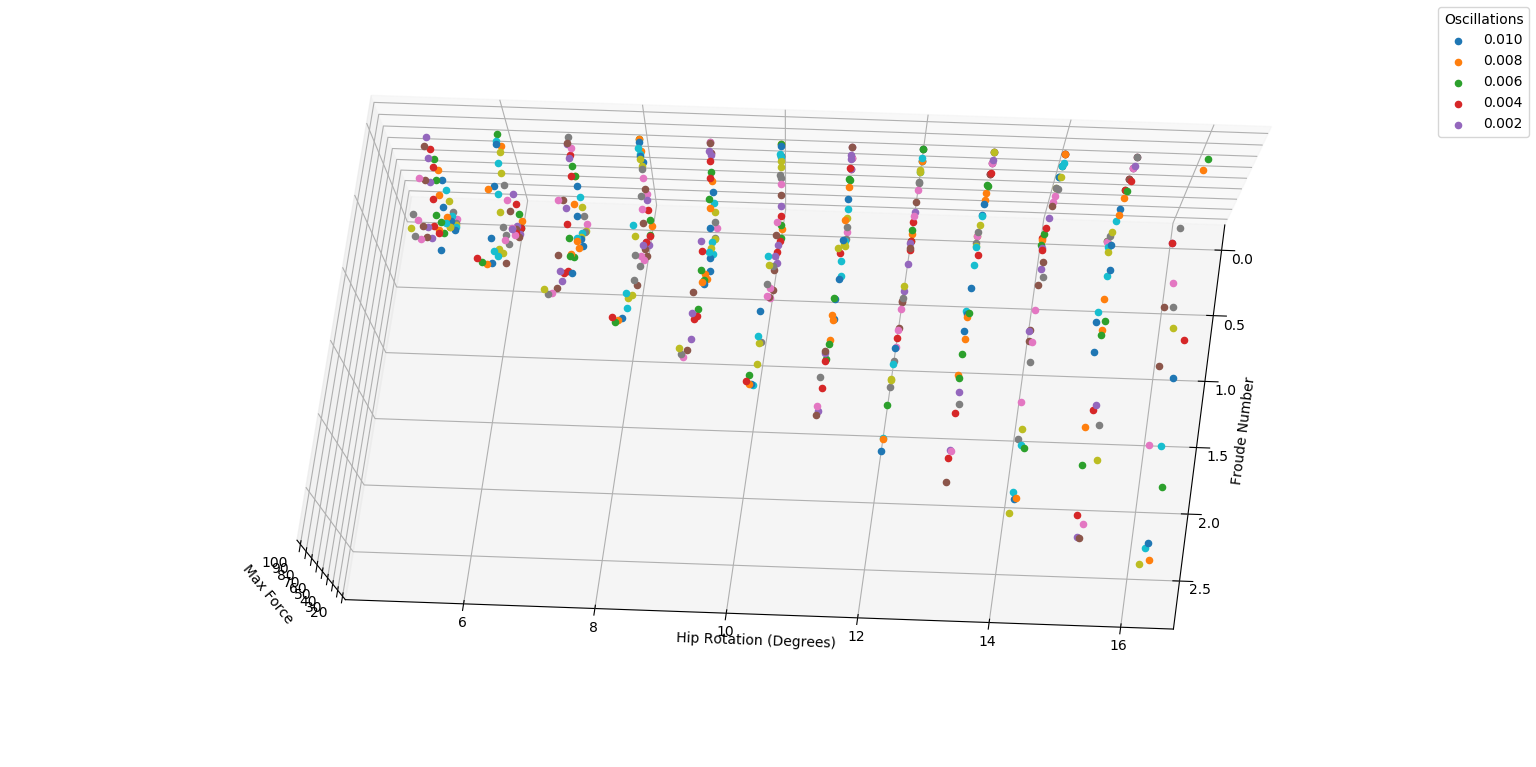
\includegraphics[width=1\textwidth]{figures/forcerotationfroude2.png}
    \label{froudenumbervsangle}
    \caption{All variation of experiments shown on 3D gragh, view 2}
\end{figure}

\begin{figure}[h!]
  \centering
  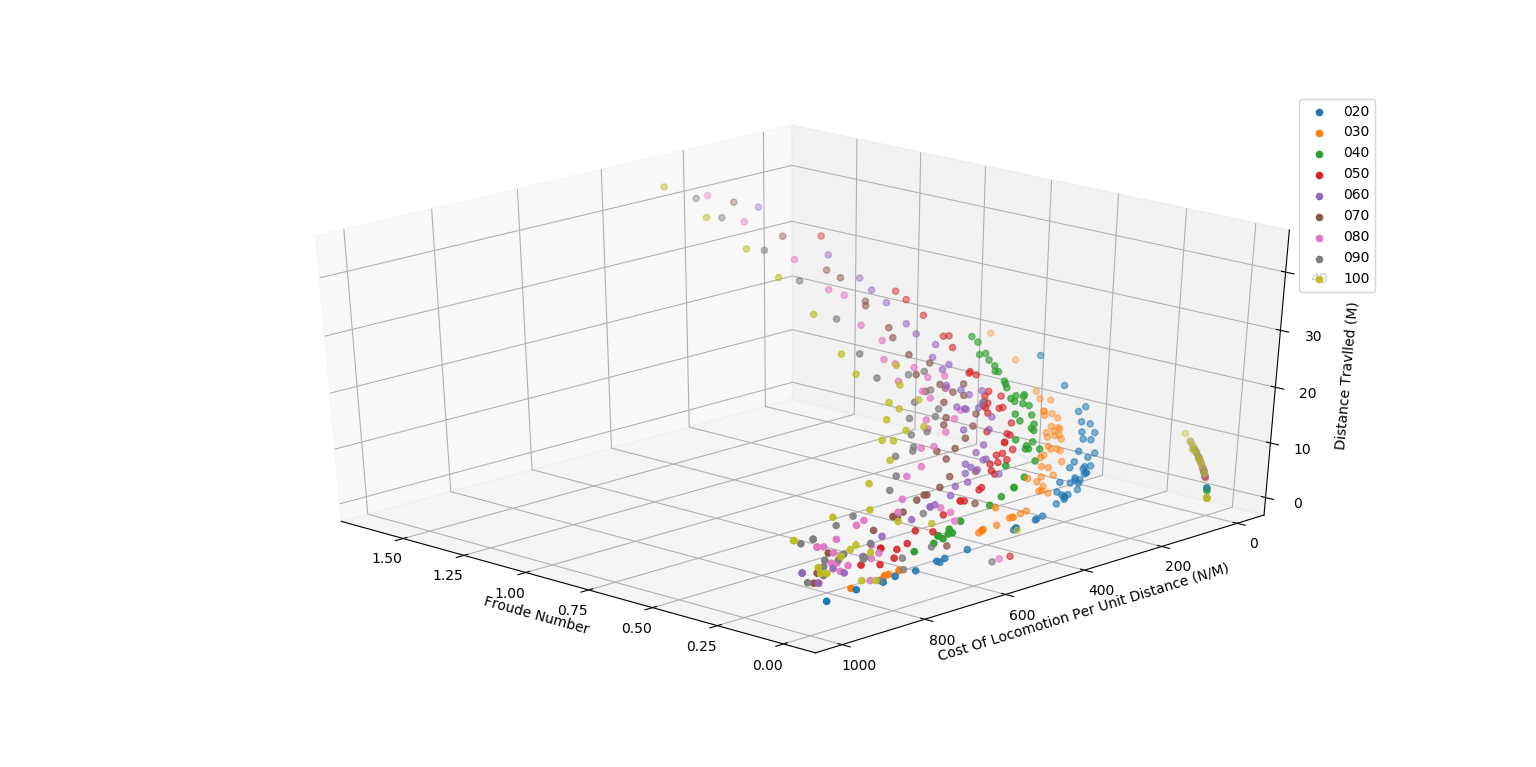
\includegraphics[width=1\textwidth]{figures/3dgraph.png} 
  \caption{Cost Of Locomotion against force applied, distance travelled on Y.}
  \label{3dgraph1}
\end{figure}

\begin{figure}[h!]
  \centering
  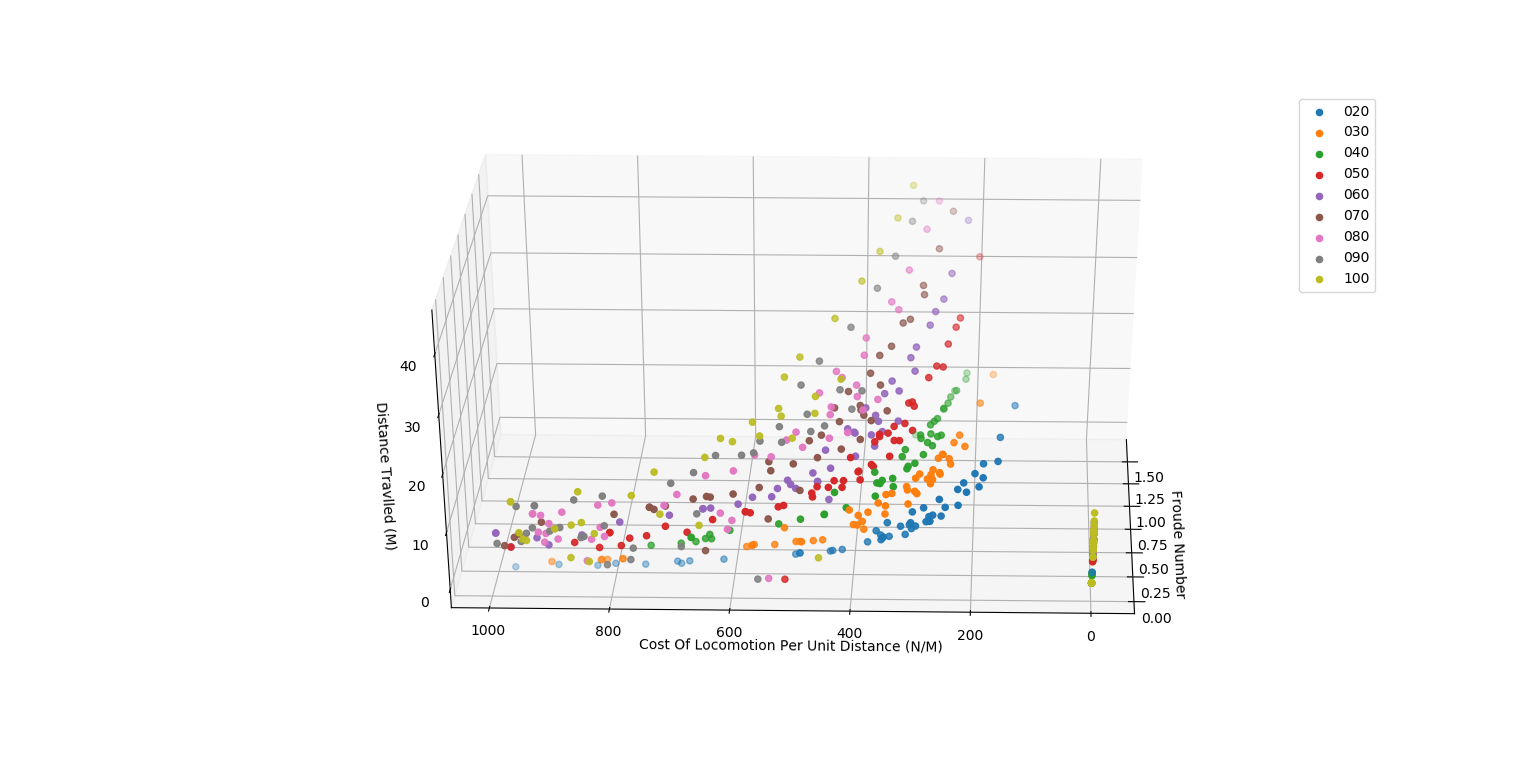
\includegraphics[width=1\textwidth]{figures/3dgraph2.png}
  \caption{Cost Of Locomotion against force applied, distance travelled on Y view 2.}
  \label{3dgraph2}
\end{figure}

\begin{figure}[h!]
  \centering
  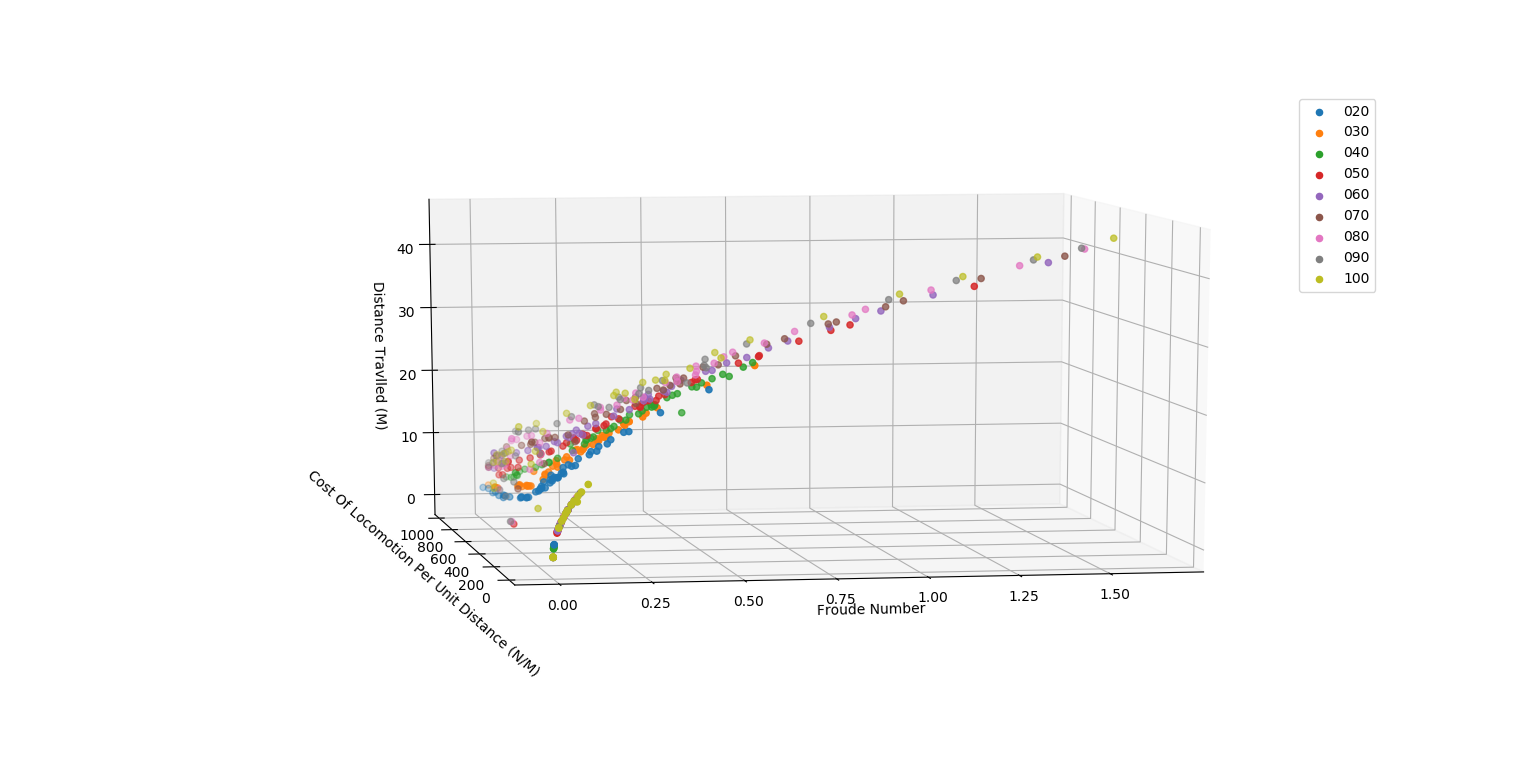
\includegraphics[width=1\textwidth]{figures/3dgraph3.png}
  \caption{Cost Of Locomotion against force applied, distance travelled on Y view 3.}
  \label{3dgraph2}
\end{figure}
